\subsection{Visual Spacing Scenario}
\begin{tikzpicture}

\foreach \x in {0,1,2,3,4}
    \draw (\x cm,0.0) -- (\x cm, 5);
    
\draw [line width=10] (0,1.175) -- (1,1.175);
\draw [line width=10] (1,2.175) -- (2,2.175);
\draw [line width=10] (2,3.175) -- (3,3.175);
\draw [line width=10] (3,4.175) -- (4,4.175);

\draw [decorate,decoration={brace,amplitude=7pt}](-0.1,1) -- (-0.1,3);
\draw [decorate,decoration={brace,amplitude=7pt}](-0.1,3) -- (-0.1,4);

\foreach \x in {3,4}
    \draw [dotted](0,\x) -- (\x,\x);

\draw (-1, 2) node {1/2};
\draw (-1, 3.5) node {1/4};

\draw [<-] (4.0,1) -- (4.5,1) node [anchor=west, xshift=0.5] {\textcolor{darkgreen}{1.0x}};

\end{tikzpicture}
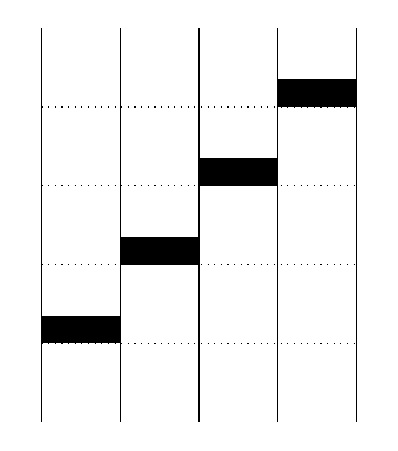
\begin{tikzpicture}

\foreach \x in {0,1,2,3,4}
    \draw (\x cm,0.0) -- (\x cm, 5);
    
\draw [line width=10] (0,1.175) -- (1,1.175);
\draw [line width=10] (1,2.175) -- (2,2.175);
\draw [line width=10] (2,3.175) -- (3,3.175);
\draw [line width=10] (3,4.175) -- (4,4.175);

\foreach \x in {1,2,3,4}
    \draw [dotted](0,\x) -- (4,\x);

\end{tikzpicture}

\noindent
\textbf{Gameplay View} (left) vs. \textbf{Editor View} (right)\newline
\textit{Each dotted line in Editor View represents} $1/4$\newline